\documentclass{article}
\def\ntitle {SIAM's Gene Golub Summer School 2013 : Function of
Matrices} \def\nauthor {Taught by Professor Nicholas J. Higham \\
Zhengbo Zhou}
\def\needcrop{ } % crop for easy previewing
\def\fancysec{ } % section font become fancier 
\RequirePackage{etex}
\makeatletter
\ifx \nauthor\undefined
  \def\nauthor{Zhengbo Zhou}
\else 
\fi 
\ifx \ndate\undefined 
  \def\ndate{\today}
\else 
\fi 

\author{\nauthor \thanks{%
Department of Mathematics,
University of Manchester,
Manchester, M13 9PL, England
(\texttt{zhengbo.zhou@postgrad.manchester.ac.uk}).
}}
\date{\ndate}
\title{\ntitle}

% RedeclareMathOperator
\newcommand\RedeclareMathOperator{%
  \@ifstar{\def\rmo@s{m}\rmo@redeclare}{\def\rmo@s{o}\rmo@redeclare}%
}
% this is taken from \renew@command
\newcommand\rmo@redeclare[2]{%
  \begingroup \escapechar\m@ne\xdef\@gtempa{{\string#1}}\endgroup
  \expandafter\@ifundefined\@gtempa
     {\@latex@error{\noexpand#1undefined}\@ehc}%
     \relax
  \expandafter\rmo@declmathop\rmo@s{#1}{#2}}
% This is just \@declmathop without \@ifdefinable
\newcommand\rmo@declmathop[3]{%
  \DeclareRobustCommand{#2}{\qopname\newmcodes@#1{#3}}%
}
\@onlypreamble\RedeclareMathOperator

\usepackage{algorithm}
\usepackage{algpseudocode}
\usepackage{comment}
\usepackage{bookmark}
\usepackage{microtype}
\usepackage{booktabs}
\usepackage{lastpage}
\usepackage{fancyhdr}
\usepackage{amsthm}
\usepackage{mathtools}
\usepackage{enumerate}
\usepackage{mathrsfs}
\usepackage{amsfonts}
\usepackage{amssymb}
\usepackage{tcolorbox}
\usepackage{bm}
\usepackage{cancel}
\usepackage{bbm}
\usepackage{accsupp}
\usepackage{enumitem}
\usepackage{hyperref}
\usepackage[fontsize=12pt]{fontsize}
\usepackage{geometry}
\usepackage{microtype}
\usepackage{algorithm,algorithmicx,algpseudocode}

\hbadness=99999

\geometry{
  a4paper,
  textwidth=165truemm,
  textheight=240truemm,
  top=28.5truemm,
}

\let\LaTeXStandardTableOfContents\tableofcontents
\renewcommand{\tableofcontents}{%
\begingroup%
\renewcommand{\bfseries}{\sc}%
\LaTeXStandardTableOfContents%
\endgroup%
}%
\setcounter{tocdepth}{3}
\makeatletter
\renewcommand\tableofcontents{\@starttoc{toc}}
\makeatother

\hypersetup{
  hypertexnames=false, 
  colorlinks=true,
  linkcolor=blue,
  pdfauthor={Zhengbo Zhou},
  pdftitle={\ntitle},
  pdfcreator={Zhengbo Zhou via MikTeX}
}

\usepackage[hyperpageref]{backref}
\renewcommand*{\backref}[1]{}
\renewcommand*{\backrefalt}[4]{
    \ifcase #1 %
    No citations.%
    \or
    (Cited on p.~#2.)
    \else
    (Cited on pp.~#2.)
    \fi
}



\pagestyle{fancyplain}
\fancyhead[R]{{\textit{\footnotesize\nouppercase Short Course : Function of Matrices}}}
\fancyhead[L]{\footnotesize\nouppercase\leftmark}


\newtcolorbox{mybox}[1]{colback=white!90!black,colframe=white!40!black,fonttitle=\scshape\centering,title=#1}

%%% MATLAB Code From Dr. Chris Johnson 
\usepackage{color}  
\usepackage{xcolor}
\usepackage{listings}
\definecolor{codegreen}{rgb}{0,0.6,0}
\definecolor{codegray}{rgb}{0.5,0.5,0.5}
\definecolor{codepurple}{rgb}{0.58,0,0.82}
\definecolor{mygreen}{RGB}{28,172,0}
\definecolor{mylilas}{RGB}{170,55,241}
\definecolor{backcolour}{rgb}{0.95,0.95,1.92}
\lstdefinestyle{mystyle}{
	language=matlab,
    commentstyle=\color{codegreen},
    keywordstyle=\color{blue},
    numberstyle=\footnotesize\color{codegray},
    stringstyle=\color{codepurple},
    basicstyle=\linespread{1}\ttfamily\small,
    breakatwhitespace=false,
    breaklines=true,
    captionpos=b,
    keepspaces=true,
    numbers=left,
    numbersep=10pt,
    showspaces=false,
    showstringspaces=false,
    showtabs=false,
    tabsize=4,
    aboveskip=\medskipamount,
    % frame=single,
}
\lstset{style=mystyle}
\def\inline{\lstinline[basicstyle=\upshape\ttfamily]}

%% Theorems 
\newtheorem{theorem}{Theorem}[section]
\newtheorem{proposition}[theorem]{Proposition}
\newtheorem{corollary}[theorem]{Corollary}
\newtheorem{lemma}[theorem]{Lemma}
\theoremstyle{definition}
\newtheorem{definition}[theorem]{Definition}
\newtheorem{example}[theorem]{Example}
\newtheorem{remark}[theorem]{Remark}
\newtheorem*{question}{Question}
\newtheorem*{recall}{Recall}
\newtheorem*{assumption}{Assumption}
\newtheorem*{note}{Note}
\numberwithin{equation}{section}

\let\stdsection\section
\renewcommand\section{\newpage\stdsection}

%%% Paired labels
\DeclarePairedDelimiter\ceil{\lceil}{\rceil}
\DeclarePairedDelimiter\floor{\lfloor}{\rfloor} 
\DeclarePairedDelimiter\abs{\lvert}{\rvert} % |a|
\DeclarePairedDelimiter\inner{\langle}{\rangle} % <a>
\makeatletter
\let\oldabs\abs
\def\abs{\@ifstar{\oldabs}{\oldabs*}}

%%%------------------------------------------------------------------%%%

%%% vector bold
\renewcommand{\vec}[1]{\bm{#1}}

%%%------------------------------------------------------------------%%%

%%% Real and Imaginary
\RedeclareMathOperator{\Im}{\mathrm{Im}}
\RedeclareMathOperator{\Re}{\mathrm{Re}}

%%% Integrate from ... to ...       
\newcommand{\intii}{\int_{-\infty}^{\infty}}

%%% Greek Letters
% NEVER define \l for \lambda due to Polish names in BibTeX
\renewcommand{\L}{\Lambda}
\newcommand{\vL}{\varLambda}
\newcommand{\g}{\gamma}
\newcommand{\G}{\Gamma}
\newcommand{\vG}{\varGamma}
\renewcommand{\o}{\omega}
\renewcommand{\O}{\Omega}
\newcommand{\vO}{\varOmega}
\newcommand{\s}{\sigma}
\renewcommand{\S}{\Sigma}
\newcommand{\vS}{\varSigma}
\newcommand{\eps}{\varepsilon}
\newcommand{\lap}{\varDelta}

%%% Matrix Related
\newcommand{\n}{^{n}}
\newcommand{\m}{^{m}}
\newcommand{\Rn}{\R^n}
\newcommand{\mn}{^{m\times n}}
\newcommand{\nn}{^{n\times n}}
\newcommand{\tp}{^{T}} 
\newcommand{\ctp}{^{*}}
\newcommand{\inv}{^{-1}}
\DeclareMathOperator{\diag}{diag}
\DeclareMathOperator{\rank}{rank}
\DeclareMathOperator{\tr}{trace}
\DeclareMathOperator{\range}{Range}

%%%------------------------------------------------------------------%%%

%% Norms
\newcommand{\iter}[1]{^{(#1)}} % iteration
\newcommand{\gnorm}[1]{\left\|{#1}\right\|} % general norm
\newcommand{\norm}[1]{\gnorm{#1}}
\newcommand{\tnorm}[1]{\gnorm{#1}_2} % 2-norm
\newcommand{\inorm}[1]{\gnorm{#1}_\infty} % infinity norm

%%% Over the expressions
\newcommand{\wh}{\widehat}
\newcommand{\wt}{\widetilde}
\newcommand{\wb}{\overline}

%%% Calculus
\DeclareMathOperator{\grad}{\nabla}
\renewcommand{\div}{\nabla\cdot}
\DeclareMathOperator{\curl}{\nabla\times}
\newcommand{\dd}{\mathrm{d}}
\newcommand{\pp}{\partial}
\def\eu{\mathrm{e}} % euler's constant
\def\im{\mathrm{i}} % imaginary unit

%%% Citation
\def\ycite[#1#2#3#4#5]#6{\cite[$\mit{#1#2#3#4}$#5]{#6}}

%%%------------------------------------------------------------------%%%

%%% MATHBB
\newcommand{\mb}[1]{\mathbb{#1}}
\newcommand{\N}{\mb{N}}
\newcommand{\Z}{\mb{Z}} 
\newcommand{\Q}{\mb{Q}}
\newcommand{\R}{\mb{R}} 
\newcommand{\C}{\mb{C}}
\newcommand{\F}{\mb{F}}
\renewcommand{\P}{\mb{P}} % Probability
\newcommand{\E}{\mb{E}} % Expectation
\newcommand{\V}{\mb{V}} % Variance

%%% MATHCAL and MATHSCR
\newcommand{\mc}[1]{\mathcal{#1}} % For spaces 
\newcommand{\ms}[1]{\mathscr{#1}} % For sigma-algebra
\newcommand{\mf}[1]{\mathfrak{#1}}

%%%------------------------------------------------------------------%%%

%%% Stochastic Calculus
\newcommand{\ps}{$(\Omega,\ms F,\P)$}
\newcommand{\ito}{It\^o}
\DeclareMathVersion{bold}
\newcommand{\indi}{\mathbbm{1}} % indicator function
\providecommand*{\napprox}{%
  \BeginAccSupp{method=hex,unicode,ActualText=2249}%
  \not\approx
  \EndAccSupp{}%
}
\mathchardef\gang="2D
\DeclareMathOperator*{\esssup}{esssup}

\DeclareMathOperator{\law}{\mathfrak{Law}}
\newcommand{\loc}{\textup{loc}}
\newcommand{\locmart}{\mc M_{\loc}^C}
\newcommand{\locm}{\mc M_{\loc,T}^{C,0}}
\newcommand{\locmt}{\wt{\mc M}_{\loc,T}^{C,0}}
\newcommand{\nicee}[1]{\mathcal{E}_{#1}^H(B)}


\DeclareMathOperator{\sign}{diag}

\makeatother
\usepackage{tikz}
\usepackage{enumitem}
\newcommand{\subscript}[2]{$#1 _ #2$}
\def\FD{Fr\'echet Derivative} 
\def\cond{\mathrm{cond}}
\def\vG{\varGamma}
\def\sign{\mathrm{sign}}

\begin{document}
\maketitle
\tableofcontents

\section{History and Definitions}

The matrix algebra arised by Cayley and Sylvester.
\begin{itemize}
    \item Matrix algebra developed by Arthur Cayley, FRS (1821--1895) in
    his paper ``Memoir on the Theory of Matrix'' (1858).
    \item Cayley considered matrix square root is his 1858 memoir.
    \item The term ``matrix'' coined in 1850 by James Joseph Sylvester,
    FRS (1814--1897).
    \item Leguerre (1867) defines the matrix exponential via power
    series.
\end{itemize}

We can define the matrix function by substitution. Suppose we want to
define $f:\C\nn \to \C\nn$,  but not elementwise. Given $f(t)$, we can
define $f(A)$ by substituting $A$ for $t$:
\begin{equation}\notag
    \begin{aligned}
        & f(t) = \frac{1+t^2}{1-t} \quad \Rightarrow \quad f(A) = (I-A)\inv (I+A^2), \\
        & \log(1 + x) = x - x^2/2 + x^3/3 - x^4/4 + \cdots, \quad \abs{x} < 1 \\
        \Rightarrow \quad & \log(I + A) = A - A^2/2 + A^3/3 - A^4/4 + \cdots, \quad \rho(A) < 1,
    \end{aligned}
\end{equation}
where $\rho(A)$ is the spectral radius of $A$ ($\rho(A) = \max
\{\abs{\lambda} : Ax = \lambda x, \forall x \in \C\n \})$. However, we
want a more general definition that works for arbitrary $f$ and
arbitrary $A$.

\subsection{Definition via Jordan canonical form}

We can reduce any $A\in\C\nn$ into Jordan canonical form (JCF):
    \begin{equation}\label{eq.jcf}
        A = Z J Z\inv, \quad J = \diag(J_1,\dots, J_p), \quad J_k =  s
        \begin{bmatrix}
            \lambda_k & 1 &  &  \\
            & \ddots & \ddots & \\
            & & \ddots & 1 \\ 
            & & & \lambda_k
        \end{bmatrix} \in \C^{m_k \times m_k},
    \end{equation}
where $Z$ is nonsingular and $m_1 + \dots + m_p = n$. Denote by 
\begin{itemize}
    \item $\lambda_1,\dots,\lambda_s$ the distinct eigenvalues of $A$,
    \item $n_i$ is the order of the largest Jordan block in which
    $\lambda_i$ appears, which is called the \emph{index} of
    $\lambda_i$. 
\end{itemize}
We say the function $f$ is \emph{defined on the spectrum of $A$} if the
values 
\begin{equation}\notag
    f\iter{j}(\lambda_i), \quad j = 0,\dots,n_i - 1,\quad i = 1,\dots,s,
\end{equation}
exist.

\begin{definition}
    [Define via Jordan Canonical Form]\label{def.jcf} Let $f$ be defined
    on the spectrum of $A\in\C\nn$ and let $A$ have the
    JCF~\eqref{eq.jcf}. Then 
    \begin{equation}\notag
        f(A) \coloneqq Z f(J) Z\inv
    \end{equation}
    where $f(J) = \diag(f(J_1),\dots, f(J_p))$ and 
    \begin{equation}\notag
        f\left(J_k\right):=
        \begin{bmatrix}
            f\left(\lambda_k\right) & f^{\prime}\left(\lambda_k\right) & \cdots & \frac{f^{(m_k-1)}\left(\lambda_k\right)}{\left(m_k-1\right) !} \\
            & f\left(\lambda_k\right) & \ddots & \vdots \\
            & & \ddots & f^{\prime}\left(\lambda_k\right) \\
            & & & f\left(\lambda_k\right)
        \end{bmatrix}
    \end{equation}
\end{definition}

It is obvious that we require some differentiability of $f$ and it
depends on the Jordan structure. If $A$ is diagonalizable, there is no
requirement on the differentiability of $f$. Conversely, if $A$ has a
large Jordan block, then lots of derivatives are required. Also, from
the definition, we see that we actually don't need the underlying
function $f$ to be smooth at all, since we only need the function value
at $\lambda_i$.

\subsubsection{``Deriving'' the formula for $f(J_k)$}
Write $J_k = \lambda_k I + E_k \in \C^{m_k \times m_k}$. For $m_k = 3$,
we have 
\begin{equation}\notag
    E_k = 
    \begin{bmatrix}
        0 & 1 & 0 \\ 0 & 0 & 1 \\ 0 & 0 & 0
    \end{bmatrix},
    E_k^2 = 
    \begin{bmatrix}
        0 & 0 & 1 \\ 0 & 0 & 0 \\ 0 & 0 & 0 
    \end{bmatrix},
    E_k^3 = 0.
\end{equation}
Assuming $f$ has Taylor expansion, then 
\begin{equation}\notag
    f(t) = f(\lambda_k) + f'(\lambda_k)(t-\lambda_k) + \cdots + \frac{f\iter{j}(\lambda_k)(t-\lambda_k)^j}{j!} + \cdots,
\end{equation}
then 
\begin{equation}\notag
    f(J_k) = f(\lambda_k)I + f'(\lambda_k)E_k + \cdots + \frac{f\iter{m_k - 1}(\lambda_k)E_k^{m_k - 1}}{(m_k - 1)!},
\end{equation}
which is exactly the expression of $f(J_k)$.

\subsection{Definition via Interpolation}
For $A\in\C\nn$, the following definition is studied by Sylvester (1886,
distinct eigenvalues) and Buckheim (1886, general eigenvalues).
\begin{definition}
    [Define via Hermite Interpolation] Given $A\in\C\nn$ which has $s$
    distinct eigenvalues $\lambda_1,\dots,\lambda_s$ and $n_i$ is the
    index of $\lambda_i$. Then $f(A) = p(A)$ where $p$ is the unique
    Hermite interpolating polynomial of degree less than $\sum_{i = 1}^s
    n_i$ satisfying: for each eigenvalue $\lambda_k$, 
    \begin{equation}\notag
        p\iter{j}(\lambda_k) = f\iter{j}(\lambda_k),\quad j = 0,\dots,n_k - 1.
    \end{equation}
\end{definition}

\begin{example}
    Let $f(t) = t^{1/2}$, $A = \begin{bmatrix} 2 & 2 \\ 1 & 3
    \end{bmatrix}$ and $\lambda(A) = \{1,4\}$. Then taking the positive
    roots, we have 
    \begin{equation}\notag
        r(t) = f(1) \frac{t-4}{1-4} + f(4)\frac{t-1}{4-1} = \frac{1}{3}(t+2),
    \end{equation}
    which gives 
    \begin{equation}\notag
        A^{1/2} = r(A) = \frac{1}{3}(A + 2I) = \frac{1}{3}
        \begin{bmatrix} 4 & 2 \\ 1 & 5 \end{bmatrix}
    \end{equation}
\end{example}

\begin{note}
    This definition gives a unique polynomial to define $f(A)$. Suppose
    we impose further interpolation conditions which may have nothing
    todo with the eigenvalues, then we gain a higher degree polynomial
    but it still interpolates the eigenvalues and it still gives the
    same result. 
    
    For example, suppose we interpolates not only $f(1) = 1$ and $f(4) =
    2$, but also $f(-1) = 5$. Then we have 
    \begin{equation}\notag
        r(t) = \frac{(t-4)(t+1)}{-6} + \frac{2(t-1)(t+1)}{15} + \frac{(t-1)(t-4)}{2},
    \end{equation}
    and we can define
    \begin{equation}\notag
        r(A) = \frac{(A-4I)(A+I)}{-6} + \frac{2(A-I)(A+I)}{15} + \frac{(A-I)(A-4I)}{2} = \frac{1}{3} \begin{bmatrix} 4 & 2 \\ 1 & 5 \end{bmatrix}
    \end{equation}
    which is exactly the same as using only 2 interpolating data.
    Further interpolating conditions wouldn't change the resul, this can
    be useful if we don't know the Jordan form. For example, we can look
    for the worst case Jordan form and get the interpolating polynomial
    using lots of data points where some of them my not necessary, but
    we will eventually get the same result.
\end{note}

The following are properties of matrix function that can be seen by
using the definition by interpolation.
\begin{itemize}
    \item $f(A)$ is a polynomial in $A$, but the polynomial depends on
    $A$.
    \item $f(A)$ commutes with $A$, i.e. $Af(A) = f(A) A$.
    \item $f(A\tp) = (f(A))\tp$. However, $f(A\ctp) \neq (f(A))\ctp$ in
    general.
\end{itemize}

The usual Cayley-Hamilton Theorem states
\begin{equation}\notag
    p(t) = \det(tI - A) \text{ implies } p(A) = 0.
\end{equation}
A generalized version of the Cayley-Hamilton theorem is
\begin{theorem}
    [Cayley, 1857] If $A, B \in \C\nn$, $AB = BA$, and $f(x,y) = \det
    (xA - yB)$, then $f(B,A) = 0$.
\end{theorem}

Using the Cayley-Hamilton theorem, $A^n$ can be expressed as a linear
combination of lower powers of $A$: $A^n = \sum_{k = 0}^{n-1}c_kA^k$.
Using this relation recursively, any power series collapses to a
polynomial. For example, $\eu^A = \sum_{k = 0}^\infty A^k/k! =
\sum_{k=0}^{n-1}d_kA^k$ where $d_k$ may depends on $A$.

\subsection{Definition via Cauchy Integral Formula}

\begin{definition}
    [Define via Cauchy Integral Formula] For $A\in\C\nn$, 
    \begin{equation}\notag
        f(A) = \frac{1}{2\pi \im}\int_\vG f(z)(zI - A)\inv ~\dd z,
    \end{equation}
    where $f$ is analytic on and inside a closed contour $\vG$ that
    enclose $\lambda(A)$.
\end{definition}

This definition is useful computationally. Suppose we would like to
compute $f(A)b$ for $A$ is large and sparse, then 
\begin{equation}\notag
    f(A)b = \frac{1}{2\pi\im}\int_{\vG} f(z)(zI - A)\inv b~\dd z.
\end{equation}
As long as we are able to solve $(zI - A)\inv b$ which is a linear
system with shifted $A$, then we are able to do quadrature here.

\subsection{Defintion via Schwerdtfeger's formula}

\begin{definition}
    [Schwerdtfeger, 1938] For $A$ with distinct eigenvalues
    $\lambda_1,\dots,\lambda_s$ with indices $n_i$, 
    \begin{equation}\notag
        f(A) = \sum_{i=1}^s A_i \sum_{j=0}^{n_i-1}\frac{f\iter{j}(\lambda_i)}{j!}(A-\lambda_i I)^j = \sum_{i=1}^s \sum_{j=0}^{n_i - 1}f\iter{j}(\lambda_i)Z_{ij},
    \end{equation}
    where $A_i$ are Frobenius covariants and $Z_{ij}$ depends on $A$ but
    not $f$. 
\end{definition}

\subsection{Equivalence of Definition}

\begin{theorem}
    The four definitions are equivalent, modulo analyticity assumption
    for the Cauchy definition.
\end{theorem}

\begin{remark} \ 
    \begin{itemize}
        \item Interpolation: For basic properties such as $A$ and $f(A)$
        commute.
        \item JCF: Solving matrix equations, e.g. $X^2 = A, \eu^X = A$
        and $W\eu^W =A$ where $W$ is the Lambert $W$ function.
        \item For computation, there exists methods that specific to
        particular $f$ and $A$.
    \end{itemize}
\end{remark}

\subsection{Primary and Nonprimary Functions}

\subsubsection{Root Oddities}
Notice that identity matrix has strange roots
\begin{itemize}
    \item $B_n^2 = I_n$ where 
    \begin{equation}\notag
        B_4 = \begin{bmatrix}
            1 & 1 & 1 & 1 \\ 0 & -1 & -2 & -3 \\
            0 & 0 & 1 & 3 \\ 0 & 0 & 0 & -1 
        \end{bmatrix}.
    \end{equation}
    This arises in backward differentiation formula solvers for ODEs.
    \item Turnbull (1927): $A^3_n = I_n$, where 
    \begin{equation}\notag
        A_4 = 
        \begin{bmatrix}
            -1 & 1 & -1 & 1 \\ -3 & 2 & -1 & 0 \\ -3 & 1 & 0 & 0 \\
            1 & 0 & 0 & 0
        \end{bmatrix}.
    \end{equation}
    \item $C_n^2 = I_n$, where
    \begin{equation}\notag
        C_n = 2^{-3/2}
        \begin{bmatrix}
            1 & 3 & 3 & 1 \\ 1 & 1 & -1 & -1 \\ 1 & -1 & -1 & 1 \\ 
            1 & -3 & 3 & -1
        \end{bmatrix}.
    \end{equation}
\end{itemize}

\subsubsection{Nonprimary Matrix Functions}
Consider the Jordan form definition~\ref{def.jcf}. However, for example
$f(t) = t^{1/2}$, we could take different square root (positive and
negative square root) for the same eigenvalues (but different Jordan
blocks). Formally, if $A$ is derogatory, and a different branch of $f$
is taken in the two different Jordan blocks for $\lambda$, we obtain a
nonprimary matrix function for $A$. For example,
\begin{equation}\notag
    \begin{aligned}
        I_2 & = 
        \begin{bmatrix}
            1 & 0 \\ 0 & 1
        \end{bmatrix}^2 = 
        \begin{bmatrix}
            -1 & 0 \\ 0 & -1 
        \end{bmatrix}^2, \quad \text{primary} \\
        & = 
        \begin{bmatrix}
            1 & 0 \\ 0 & -1 
        \end{bmatrix}^2 = 
        \begin{bmatrix}
            \cos(\theta) & \sin(\theta) \\ \sin(\theta) & -\cos(\theta)
        \end{bmatrix}^2, \quad \text{non-primary.}
    \end{aligned}
\end{equation}

Primary matrix functions are expressible as a polynomial in $A$, while
nonprimary ones are not. Therefore the above three examples are all
nonprimary matrix square roots of $I_2$.

Sometimes, the nonprimary function are interested. For example, we would
like to find the square root of rotations $G(\theta)$ where 
\begin{equation}\notag
    G(\theta) = 
    \begin{bmatrix}
        \cos(\theta) & \sin(\theta) \\ -\sin(\theta) & \cos(\theta)
    \end{bmatrix}.
\end{equation}
Apparently, $G(\theta/2)$ is a natural square root of $G(\theta)$.
However, for $\theta = \pi$,
\begin{equation}\notag
    G(\pi) = 
    \begin{bmatrix}
        -1 & 0 \\ 0 & -1
    \end{bmatrix}, \quad 
    G(\pi/2) = 
    \begin{bmatrix}
        0 & 1 \\ 0 & -1
    \end{bmatrix},
\end{equation}
which implies $G(\pi/2)$ is a nonprimary square root of $G(\pi)$.

Sometimes, the family of all nonprimary matrix functions can be written
explicitly. For example, we would like to find a matrix $X$ such that 
\begin{equation}\notag
    X^2 = A = 
    \begin{bmatrix}
        1 & 1 & 0 \\ 0 & 1 & 0 \\ 0 & 0 & 1
    \end{bmatrix}.
\end{equation}
A solution is 
\begin{equation}\notag
    X = 
    \begin{bmatrix}
        1 & 1/2 & 0 \\ 0 & 1 & 0 \\ 0 & 0 & 1
    \end{bmatrix}.
\end{equation}
In fact, all square roots of $A$ are given by 
\begin{equation}\notag
    Y = \pm U 
    \begin{bmatrix}
        1 & 1/2 & 0 \\ 0 & 1 & 0 \\ 0 & 0 & -1 
    \end{bmatrix}
    U\inv, \quad U =  
    \begin{bmatrix}
        a & b & d \\ 0 & a & 0 \\ 0 & e & c
    \end{bmatrix}
\end{equation}
where $a,b,c,d$ and $e$ are any numbers that make $U$ nonsingular.

\subsection{Principal Logarithm, root and power}
Notice that suppose $X$ is a solution of $\eu^X = A$, then $X + 2\alpha
\pi \im I$ for all $\alpha \in \Z$ is a solution of $\eu^X = A$.
Therefore, we need to make a choice on the solutions.

Let $A\in\C\nn$ have no eigenvalues on $\R_-$, 
\begin{definition}
    [Principal Log] $X = \log(A)$ denotes the unique $X$ such that 
    \begin{itemize}
        \item $e^X = A$,
        \item $-\pi < \Im(\lambda(X)) < \pi$.
    \end{itemize}
\end{definition}

\begin{definition}
    [Principal $p$th root] For integer $p > 0$, $X = A^{1/p}$ is the
    unique $X$ such that 
    \begin{itemize}
        \item $X^p = A$,
        \item $-\pi/p < \mathrm{arg}(\lambda(X)) < \pi/p$.
    \end{itemize}
\end{definition}

\begin{definition}
    [Principal power] For $s \in \R$, $A^s = \eu^{s\log A}$, where $\log
    A$ is the principal logarithm. It also have the integral
    representation:
    \begin{equation}\notag
        A^s = \frac{\sin(s\pi)}{s\pi}A \int_0^\infty (t^{1/s}I + A)\inv~\dd t, \quad s \in (0,1).
    \end{equation}
\end{definition}

\section{Application}
\subsection{Toolbox of Matrix Functions}
In software, we want to be able to evaluate interesting $f$ at matrix
arguments as well as scalar arguments. For example, trigonometric matrix
functions, as well as matrix roots. For the second order differential
equation,
\begin{equation}\notag
    \frac{\dd^2 y}{\dd t^2} + Ay = 0,\quad y(0) = y_0, \quad y'(0) = y'_0
\end{equation}
has solution 
\begin{equation}\notag
    y(t) = \cos(\sqrt{A}t) y_0 + (\sqrt{A})\inv \sin(\sqrt{A}t)y'_0,
\end{equation}
where $\sqrt{A}$ denotes any square root of $A$. On the other hand, the
differential equation can be convert to a first order system and solved
using the exponential:
\begin{equation}\notag
    \begin{bmatrix} y' \\ y \end{bmatrix} = 
    \exp \left(
        \begin{bmatrix}
            0 & -tA \\ tI_n & 0
        \end{bmatrix}
    \right)
    \begin{bmatrix} y'_0 \\ y_0 \end{bmatrix}.
\end{equation}

MATLAB has several preinstalled functions that can take matrix as input,
e.g. \texttt{funm}, \texttt{expm}, \texttt{logm} and  \texttt{sqrtm}.

\subsection{Linear Constant Coefficient ODE}
In nuclear magnetic resonance (NMR) spectroscopy Solomon equations 
\begin{equation}\notag
    \frac{\dd M}{\dd t} = -RM, \quad M(0) = I
\end{equation}
where $M(t)$ is a matrix of intensities and $R$ is a symmetric
relaxation matrix. Thus $M(t) = \eu^{-Rt}$.

Burnup calculations in nuclear reactor analysis involve 
\begin{equation}\notag
    \frac{\dd X}{\dd t} = AX, \quad X(0) = X_0,
\end{equation}
where $A$ is often upper triangular.

\subsection{Application to Complex Networks}
Adjacency matrix of the following undirected network:

\begin{center}
    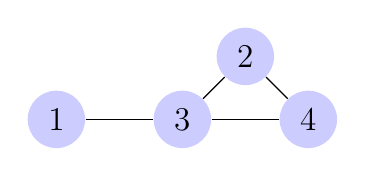
\begin{tikzpicture}
        [scale=.8,auto=left,every node/.style={circle,fill=blue!20}]
        \node (1) at (0,0) {1}; \node (2) at (3,1)  {2}; \node (3) at
        (2,0)  {3}; \node (4) at (4,0) {4};
      
        \foreach \from/\to in {1/3,3/2,3/4,2/4} \draw (\from) -- (\to);
    \end{tikzpicture}
\end{center}
gives 
\begin{equation}\notag
    A = 
    \begin{bmatrix}
        0 & 0 & 1 & 0 \\ 0 & 0 & 1 & 1 \\ 1 & 1 & 0 & 1 \\ 0 & 1 & 1 & 0
    \end{bmatrix}.
\end{equation}

\begin{definition}
    [Network measures]\

    \begin{itemize}
        \item Centrality: $(\eu^A)_{ii}$ measures how important node $i$
        is,
        \item Communicability: $(\eu^A)_{ij}$ measures how well
        information is transferred between nodes $i$ and $j$.
    \end{itemize}
\end{definition}

\begin{remark}
    \
    \begin{itemize}
        \item We can use the resolvent $(I - \alpha A)\inv$ in place of
        $\eu^A$.
        \item $\tr(\cosh(A))/\tr(\eu^A)$ is a measure of how close a
        graph is to bipartite.
    \end{itemize}
\end{remark}

\subsection{The Average Eye}
First order character of optical systtem characterized by
\emph{transference} matrix 
\begin{equation}\notag
    T = \begin{bmatrix}
        S & \delta \\ 0  & 1
    \end{bmatrix}\in \R^{5\times 5}
\end{equation}
where $S \in \R^{4\times 4}$ is symplectic:
\begin{equation}\notag
    S\tp J S = J = \begin{bmatrix}
        0 & I_2 \\ -I_2 & 0
    \end{bmatrix}.
\end{equation}
The usual average $m^{-1}\sum_{i=1}^mT_i$ is not a transference matrix.
Harris(2005) propose the average $\exp(m^{-1}\sum_{i=1}^m\log(T_i))$
which is always a transference matrix. 

\subsection{Random Multivariate Samples in Statistics}
When we sample from $N(\mu,C)$, we normally sample $x\in N(0,I)$, then
compute the Cholesky factorization of $C = LL\tp$, then $y = \mu + Lx
\sim N(\mu,C)$, $C\in\R^{m\times m}$. In some applications, $C$ has
dimension greater than $10^{12}$ and computing the Cholesky factor is
impractical. Chen, Anitescu and Saad propose that $y = \mu + C^{1/2}x
\sim N(\mu,C)$. This is practical since we only need to compute
$C^{1/2}x$ instead of compute $C^{1/2}$ explicitly, and $C^{1/2}x$ can
be computed via such as Krylov method.




\section{Properties}
We present some basic properties of matrix functions.

\begin{enumerate}[label=(\subscript{P}{{\arabic*}})]
    \item $f(XAX\inv) = Xf(A)X\inv$. This is immediate from the Jordan
    form definition, since similar matrices can be taken to have the
    same Jordan form. This is also immediate from $f(A)$ is a polynomial
    of $A$, then $f(XAX\inv) = Xf(A)X\inv$ comes from $(XAX\inv)^k =
    XA^kX\inv$.
    \item Eigenvalues of $f(A)$ are $f(\lambda_i)$, where the
    $\lambda_i$ are the eigenvalues of $A$. Notice that $A$ and $f(A)$
    are not necessarily have the same Jordan form. For example, define
    the sign function
    \begin{equation}\notag
        \sign(z) = 
        \begin{cases}
            1 & \Re(z)\geq 0, \\ -1 & \Re(z) \leq 0,
        \end{cases}
    \end{equation}
    then $\sign(A) = Z \diag(\sign(\lambda_i))Z\inv$ where the large
    Jordan block collapses into several $1\times 1$ Jordan block.
    \item If $A = (A_{ij})$ is a block triangular, then $F = f(A)$ is
    block triangular with the same block structure as $A$, and $F_{ii} =
    f(A_{ii})$.
    \item If $D = \diag(D_{ii})$, then $f(D) = \diag(f(D_{ii}))$.
    \item If $h = f+g$, then $h(A) = f(A) + g(A)$; if $h(t) = f(g(t))$,
    then $h(A) = f(g(A))$.
    \item Polynomial functional relations generalize from the scalar
    cases. If $$G(f_1,\dots,f_m) = 0, $$ where $G$ is a polynomial, then
    $G(f_1(A),\dots, f_m(A)) = 0$, such as 
    \begin{equation}\notag
        \begin{aligned}
            & \sin^2(A) + \cos^2(A) = I, \\
            & (A^{1/p})^p = A \quad \text{for any integer $p > 0$,}\\
            & \eu^{\im A} = \cos(A) + \im \sin(A).
        \end{aligned}
    \end{equation}
    \item Some relations can fail:
    \begin{itemize}
        \item $f(A\ctp) \neq (f(A))\ctp$ in general,
        \item $\eu^{\log(A)} = A$ but $\log(\eu^A) \neq A$ in general
        since it requires $A$'s eigenvalues lie between $\pm \pi$.
        \item $(AB)^{1/2} \neq A^{1/2} B^{1/2}$ in general.
        \item $\eu^A \neq (\eu^{A/\alpha})^{\alpha}$ in general. This is
        true for $\alpha \in \R_+$. 
        \item $\eu^{(A+B)t} = \eu^{At}\eu^{Bt}$ for all $t$ if and only
        if $AB = BA$.
    \end{itemize}
\end{enumerate}

\subsection{Function of Triangular Matrices}

\begin{example}
    [Function of $2\times 2$ triangular matrix]
    \begin{equation}\notag
        f\left(
        \begin{bmatrix}
            \lambda_1 & t_{12} \\ & \lambda_2
        \end{bmatrix}
        \right) = 
        \begin{bmatrix}
            f(\lambda_1) & t_{12}f[\lambda_1,\lambda_2] \\ 0 & f(\lambda_2)
        \end{bmatrix},
    \end{equation}
    where 
    \begin{equation}\notag
        f[\lambda_1,\lambda_2] = 
        \begin{cases}
            \displaystyle \frac{f(\lambda_2) - f(\lambda_1)}{\lambda_2 - \lambda_1}, & \lambda_1 \neq \lambda_2 \\
            f'(\lambda_1), & \lambda_1 = \lambda_2.
        \end{cases}
    \end{equation}
    \begin{proof}
        Using the fact that $T = \begin{bmatrix} \lambda_1 & t_{12} \\ 0
        & \lambda_2 \end{bmatrix}$ commute with $F = f(T) =
        \begin{bmatrix} f(\lambda_1)  & F_{12} \\ 0 & f(\lambda_2)
        \end{bmatrix}$ (this structure is by property $P_2$ and $P_3$),
        we have 
        \begin{equation}\notag
            \begin{bmatrix} \lambda_1 & t_{12} \\ 0 & \lambda_2 \end{bmatrix}
            \begin{bmatrix} f(\lambda_1)  & F_{12} \\ 0 & f(\lambda_2) \end{bmatrix} = 
            \begin{bmatrix} f(\lambda_1)  & F_{12} \\ 0 & f(\lambda_2) \end{bmatrix}
            \begin{bmatrix} \lambda_1 & t_{12} \\ 0 & \lambda_2 \end{bmatrix}.
        \end{equation}
        By looking at the $(1,2)$ entry, we have 
        \begin{equation}\notag
            \lambda_1 F_{12}+ t_{12} f(\lambda_2) = f(\lambda_1)t_{12} + F_{12}\lambda_2
        \end{equation}
        gives 
        \begin{equation}\notag
            F_{12} = \frac{f(\lambda_1) - f(\lambda_2)}{\lambda_1 - \lambda_2} t_{12},
        \end{equation}
        which proves the claim.
    \end{proof}
\end{example}

\begin{theorem}
    [Davis, 1973; Descloux, 1963; Van Loan, 1975] If $T$ is upper
    triangular, so is $F = f(T)$ and $f_{ii} = f(t_{ii})$, 
    \begin{equation}\notag
        f_{ij} = \sum_{(s_0,\dots,s_k) \in S_{ij}} t_{s_0,s_1}t_{s_1,s_2}\cdots t_{s_{k-1},s_k} f[\lambda_{s_0}, \dots, \lambda_{s_k}],
    \end{equation}
    where $\lambda_i = t_{ii}$.
    \begin{itemize}
        \item $S_{ij}$ is the set of all strictly increasing sequences
        of integers starting at $i$ and ending at $j$. For example,
        $S_{14} = \{(1,4),(1,2,4),(1,3,4),(1,2,3,4)\}$, and 
        \item $f[\lambda_{s_0}, \dots, \lambda_{s_k}]$ is the $k$th
        order divided difference function.
    \end{itemize}
\end{theorem}

\textbf{Problem of this formula}:
\begin{enumerate}
    \item Complexity of evaluating via computer is increasing
    exponentially,
    \item hard/tricky to implement the divided difference function.
\end{enumerate}

\subsection{Diagonalizable Matrices}
How to prove $\sin^2(A) + \cos^2(A) = I$?

\begin{theorem}
    Let $\mc D$ be an open subset of $\R$ or $\C$ and let $f$ be $n-1$
    times continuously differentiable on $\mc D$. Then $f(A) = 0$ for
    all $A\in\C\nn$ with spectrum in $\mc D$ if and only if $f(A) = 0$
    for all diagonalizable matrix $A\in\C\nn$ with spectrum in $\mc D$.
\end{theorem}

Using this theorem, $\sin^2(A) + \cos^2(A) = I$ is trivial. And it can
be used to prove the following theorem:

\begin{theorem}
    For $A\in\C\nn$ with no eigenvalues on $\R^-$,
    \begin{equation}
        \log(A) = \int_0^1 (A - I)\left(t(A - I)+I\right)\inv~\dd t.
    \end{equation}
\end{theorem}

\section{\FD\ and Condition Number}

\begin{definition}
    [\FD] The \FD\ of a matrix function $f:\C\nn \to \C\nn$ at a point
    $X\in\C\nn$ is a linear mapping $L:\C\nn \to \C\nn$ such that for
    all $E\in\C\nn$, where $E$ is an arbitrary perturbation of $X$,
    \begin{equation}\notag
        f(X + E) - f(X) - L(X,E) = o(\norm{E}).
    \end{equation}
    \FD\ is linear in the second argument by definition.
\end{definition}

\begin{example}
    For $f(X) = X^2$, we have 
    \begin{equation}\notag
        f(X+E) - f(X) = EX + XE + E^2,
    \end{equation}
    so $L(X,E) = XE + EX$.
\end{example}

\begin{example}
    [\FD\ of $\eu^A$]
    \begin{equation}\notag
        L(A,E) = \int_0^1 \eu^{A(1-s)}E\eu^{As}~\dd s.
    \end{equation}
    This can be simplified to $L(A,E) = E\eu^{A} = \eu^{A}E$ when $AE =
    EA$. Another representation will be 
    \begin{equation}\notag
        L(A,E) = E + \frac{AE + EA}{2!} + \frac{A^2E + AEA + EA^2}{3!} + \cdots.
    \end{equation}
\end{example}

\subsection{Condition Number}

For $E$ as a perturbation of $A$, we have 
\begin{equation}\notag
    \cond(f,A) = \lim_{\epsilon \to 0}\sup_{\norm{E} \leq \epsilon \norm{A}} 
    \frac{\norm{f(A +E) - f(A)}}{\epsilon \norm{f(A)}}
\end{equation}
measures the maximum changes in $f$ subject to a small change in $A$ in
relative sense.

\begin{lemma}
    \begin{equation}\notag
        \cond(f,A) = \frac{\norm{L(A)}\norm{A}}{\norm{f(A)}},
    \end{equation}
    where 
    \begin{equation}\notag
        \norm{L(A)} \coloneqq \max_{E\neq 0} \frac{\norm{L(A,E)}}{\norm{E}}.
    \end{equation}
\end{lemma}

\begin{example}
    [Condition number of $\eu^A$]
    \begin{equation}\notag
        \kappa_{\exp}(A) = \frac{\norm{L(A)}\norm{A}}{\norm{\eu^A}}.
    \end{equation}
    Using $\norm{L(A)} \geq \norm{L(A,I)} = \norm{\eu^A}$, we have
    $\kappa_{\exp}(A) \geq \norm{A}$.
\end{example}

\begin{theorem}
    \ 
    \begin{itemize}
        \item For normal $A\in\C\nn$, $\kappa_{\exp}(A) = \tnorm{A}$.
        \item If $A\in\R\nn$ is a nonnegative scalar multiple of a
        stochastic matrix, then in the $\infty$-norm, $\kappa_{\exp}(A)
        = \inorm{A}$.
    \end{itemize}
\end{theorem}


\subsection{Computing $L_f$}

We can compute $L_f$ via $2n\times 2n$ matrix: Consider the matrix 
\begin{equation}\notag
    \begin{bmatrix}
        A & E \\ 0 & A
    \end{bmatrix} \in \C^{2n \times 2n},
\end{equation}
then 
\begin{equation}\notag
    f\left(\begin{bmatrix}
        A & E \\ 0 & A
    \end{bmatrix}\right) = 
    \begin{bmatrix}
        f(A) & L_f(A,E) \\ 0 & f(A)
    \end{bmatrix}.
\end{equation}

Note that $L_f(A,\alpha E) = \alpha L_f(A,E)$, but $\alpha$ may affect
algorithm used for the evaluation, since we can let $\alpha E$ be
arbitrarily smaller than $A$ which could lead to inaccuracy.

Instead, we can compute the $L_f$ via finite difference method, 
\begin{equation}\notag
    f'(x) = \frac{f(x+h) - f(x)}{h}.
\end{equation}
Notice that, we need a little bit of care when choosing $h$, the
accuracy will increase when $h\to 0$, but it will eventually loses its
accuracy due to cancellation error (roundoff error).

\begin{figure}[H]
    \centering
    \includegraphics[width=0.5\textwidth]{matlab/totalerror.pdf}
    \caption{The absolute error of $f'(1)$ using finite difference
    method, where $f(x) = x^2$. (See Appendix~\ref{app.fdm_error})}
    \label{fig:FDM_error}
\end{figure}

We can improve from this method by the following: assume $f:\R\nn\to
\R\nn$ and $A,E\in\R\nn$. Then 
\begin{equation}\notag
    f(A + \im hE) - f(A) - \im hL_f(A,E) = o(h).
\end{equation}
Thus (AI-Moly, Higham, 2010)
\begin{equation}\notag
    f(A) \approx \Re{f(A + \im hE)}, \qquad L_f(A,E) \approx = \Im {\left({f(A
      + \im hE)\over h}\right)}.
\end{equation}

This can be explained via Taylor expansion, 
\begin{equation}\notag
    f(X + \im hE) = f(X) + \im hL_f(A,E) - \frac{h^2}{2!}L_f\iter{2}(A,E) + \frac{ih^3}{3!}L_f\iter{3}(A,E) - \cdots
\end{equation}
where 
\begin{equation}\notag
    L_f\iter{i}(A,E) = \frac{\dd^j}{\dd t^j}f(A + tE)\mid_{t=0}.
\end{equation}
Taking the $\Im(\cdot)$, we have $\frac{f(A + \im hE)}{h}$ is an order
$\mc O(h^2)$ approximation of $L_f(A,E)$.
\begin{remark}
    \ 
    \begin{itemize}
        \item $h$ is not restricted by floating point arithmetic
        considerations.
        \item Computing $f$ must not employ complex arithmetic, e.g. we
        cannot use Schur decomposition which can arise complex values.
    \end{itemize}
\end{remark}

\subsection{Condition Estimation}
The key idea is that: $L_f$ is a \emph{linear} function of $E$. Then 
\begin{equation}\label{eq.vecandFD}
    \mathrm{vec}(L_f(A,E)) = K(A)\mathrm{vec}(E)
\end{equation}
where $K(A) \in\C^{n^2 \times n^2}$ is the Kronecker form of the \FD.

\begin{lemma}
    \begin{equation}\notag
        \norm{L_f(A)}_F = \tnorm{K(A)}.
    \end{equation}
\end{lemma}
\begin{proof}
    Notice that $\norm{A}_F = \tnorm{\mathrm{vec}(A)}$, then 
    \begin{equation}\notag
        \norm{L_f(A)}_F = \max_{E\neq 0} \frac{\norm{L_f(A,E)}_F}{\norm{E}_F} = \max_{E\neq 0} \frac{\tnorm{\mathrm{vec}(L_f(A,E))}}{\tnorm{\mathrm{vec}(E)}} = \max_{E\neq 0} \frac{\tnorm{K(A)\mathrm{E}}}{\tnorm{\mathrm{vec}(E)}}  = \tnorm{K(A)},
    \end{equation}
    by definition of 2-norm.
\end{proof}

\begin{algorithm}
    \caption{Power method applied to $A\ctp A$ to produce $\gamma \leq
    \tnorm{A}$}
    \begin{algorithmic}[1]
        \State {Choose a nonzero starting vector $z_0 \in \C\n$,}
        \For{$k = 0:\infty$} \State $w_{k+1} = Az_{k}$ \State $z_{k+1} =
        A\ctp w_{k+1}$ \State $\gamma_{k+1} =
        \tnorm{z_{k+1}}/\tnorm{w_{k+1}}$ \If {Converged} \State $\gamma
        = \gamma_{k+1}$, quit. \EndIf \EndFor
    \end{algorithmic}
\end{algorithm}
For $A = K(A)$, we would like to know how to compute $(K(A))\ctp x$ and
$K(A)x$. These quantities can be calculated using \FD\ by
\eqref{eq.vecandFD} which gives Algorithm~\ref{alg.powermethodFD}.

\begin{algorithm}[H]
    \caption{2-norm power method to produce $\gamma\leq
    \norm{L_f(A)}_F$.}\label{alg.powermethodFD}
    \begin{algorithmic}[1]
        \State Choose a starting nonzero starting matrix $Z_0 \in
        \C\nn$. \For{$k = 0:\infty$} \State $W_{k+1} = L_f(A,Z_k)$
        \State $Z_{k+1} = L_f\ctp (A,W_{k+1})$ \State $\gamma_{k+1} =
        \norm{Z_{k+1}}_F/\norm{W_{k+1}}_F$ \If {Converged} \State
        $\gamma = \gamma_{k+1}$, quit. \EndIf \EndFor
    \end{algorithmic}
\end{algorithm}
In practice, we use instead the block 1-norm estimator (Higham \&
Tisseur, 2000).

\section{Problem Classification}
\subsection{Small/Medium Scale Problem}
\begin{enumerate}
    \item Decomposition
    \begin{itemize}
        \item Normal $A$: if we can compute Schur/spectral decomposition
        $A = QDQ\ctp, D = \diag(d_i)$, then $f(A) = Q
        \diag(f(d_i))Q\ctp$.
        \item Nonnormal $A$: if we can compute Schur decomposition $A =
        QTQ\ctp$, then use Schur-Parlett method.
    \end{itemize}
    \item  Matrix iterations: $X_{k+1} = g(X_k), X_0 = A$, for matrix
    $p$th root, sign function, polar decomposition. Iterations only
    require matrix multiplication and solution of multiple right-hand
    side linear system.
    \item Approximation method: polynomial (Taylor expansion) and
    rational (Pad\'e) approximation.
\end{enumerate}
\subsection{Large Scale $f(A)b$ problem}
Assume that $A$ is large and sparse, $f(A)$ cannot be stored exactly and
the problem is $f(A)b$: action of $f(A)$ on $b$.

\textbf{Case 1.} We can solve $Ax=b$ by sparse direct methods such as
\texttt{SparseLU} in MATLAB but cannot compute the Schur decomposition:
``backslash matrix''.
\begin{itemize}
    \item Cauchy integral formula can be used (Hale, H \& Trefethen,
    2008).
    \item Rational Krylov can be used with direct solves.
\end{itemize}

\textbf{Case 2.} We can only compute matrix-vector products $Ax$ and
maybe $A\ctp x$. You may have more information of $A$ such as $A$ is
symmetric or $\lambda(A) \subseteq [\lambda_{\min}, \lambda_{\max}]$
with $\lambda_{\min}$ and $\lambda_{\max}$ known.
\begin{itemize}
    \item Krylov methods.
    \item Polynomial approximations.
\end{itemize}

\subsection{Accuracy Requirement}
\begin{itemize}
    \item Full double precision.
    \item Variable tolerance, e.g. within an ODE integrator.
    \item Given tolerance, where matrix $A$ is subject to measurement
    error, e.g. $\approx 10^{-4}$ in engineering and healthcare.
\end{itemize}

\section{Methods for $f(A)$}
This this second, we will introduce
\begin{itemize}
    \item Approximation techniques: Taylor series and Pad\'e
    approximation.
    \item Decomposition techniques: Similarity transformations and block
    diagonalizations.
    \item Iteration methods: Parlett recurrence, BH method, block
    Parlett recurrence and Schur-Parlett algorithm.
    \item Finally we analyze the Newton's method for matrix sign
    function and square root function.
\end{itemize}

\begin{mybox}
    {} Approximation Methods.
\end{mybox}

\subsection{Taylor Series}
Matrix Taylor series converges if eigenvalues of increment matrix lie
within radius of convergence of series. Thus for all $A$,
\begin{equation}\notag
    \cos(A) = I - \frac{A^2}{2!} + \frac{A^4}{4!} - \frac{A^6}{6!} + \cdots
\end{equation}
We have the bound for error in trancated Taylor series in terms of
appropriate derivative at matrix argument. However, we need some
numerical consideration of computing the truncated Taylor series.

\subsection{Pad\'e Approximation}

Rational function $r_{km}(x) = p_{km}(x)/q_{km}(x)$ is a $[k,m]$ Pad\'e
approximation to $f(x) = \sum_{i=0}^\infty \alpha_i x^i$ if $p_{km}$ and
$q_{km}$ are polynomials of degree at most $k$ and $m$ respectively, and 
\begin{equation}\notag
    f(x) - r_{km}(x) = \mc O(x^{k+m+1}).
\end{equation}
The idea is: $p_{km}$ is a polynomial of degree $k$, so it has $k+1$
degree of freedom. Similarly, $q_{km}$ has $m+1$ degree of freedom.
Therefore, we have $k+m+2$ degree of freedom in total. However, multiply
$p_{km}$ and $q_{km}$ by the same constant will not change $r_{km}$
cause the degree of freedom is actually $k+m+1$. Therefore we expect
$f(x) - r_{km}(x) = \mc O(x^{k+m+1})$ which is the first
``unconsidered'' term of the Pad\'e approximant $r_{km}(x)$.

\begin{remark}
    \ 
    \begin{itemize}
        \item This is generally more efficient than truncated Taylor
        series.
        \item Possible ways of evaluating $r_{km}(x)$
        \begin{itemize}
            \item Ratio of polynomials.
            \item Continued fractions.
            \item Partial fractions.
        \end{itemize}
    \end{itemize}
\end{remark}

\begin{mybox}
    {} Decomposition methods: Similarity transformations and block
    diagonalization.
\end{mybox}

\subsection{Similarity Transformations}
We can use the formula 
\begin{equation}\notag
    A = XBX\inv \quad\Rightarrow\quad f(A) = Xf(B)X\inv
\end{equation}
provided $f(B)$ is easy to compute. 

The problem of this method is that, any error in $f(B)$ will be
magnified by a factor up to $\kappa(X) = \norm{X}\norm{X\inv}$: Consider
$A = XBX\inv$ and $f(A) = Xf(B) X\inv$. Suppose we have our computed
$f(A)$ as $\wt F = X(f(B) + \varDelta B)X\inv$, where $\norm{\varDelta
B} \approx u\norm{B}$. Then we have $\wt F = f(A) + \varDelta F$, where 
\begin{equation}\notag
    \norm{\varDelta F} \leq u \norm{B} \kappa(X).
\end{equation}
The matrix $X$ can be ill-conditioned which leads to a large error in
computed $f(A)$. This is why we prefer unitary $X$, thus we can use 
\begin{itemize}
    \item Eigendecomposition (diagonal $B$) when $A$ is normal.
    \item Schur decomposition (triangular $B$) in general $A$.
\end{itemize}

\begin{example}
    Suppose we have our \texttt{funm\_ev}
\begin{lstlisting}[numbers=none]
    function F = funm_ev(A,fun) 
    [V,D] = eig(A); 
    F = V * diag(feval(fun,diag(D))) / V;
\end{lstlisting}
Then we compare the error
\begin{lstlisting}[numbers=none]
    >> A = [3,-1;1,1]; X = funm_ev(A,@sqrt) 
    X = 
        1.7678e+00  -3.5355e-01
        3.5355e-01   1.0607e+00 
    >> norm(A-X*X)      % cond(V) =  9.5e7
    ans = 
        2.3067e-08 
    >> Y = sqrtm(A); norm(A-Y*Y) 
    ans = 
        6.4855e-16
\end{lstlisting}
\end{example}

\subsection{Block Diagonalization}
We could find a intermediate solution between the Schur form and
completely diagonalizing the matrix is the block diagonalization $A =
XDX\inv$, where 
\begin{itemize}
    \item $X$ is well conditioned.
    \item $D = \diag(D_{ii})$ is block diagonal.
\end{itemize}
We start from a Schur decomposition $A = QTQ\ctp$, then we do further
work to compute a block diagonal matrix $D = XTX\inv = \diag(D_{ii})$
where $\kappa(X) < tol$. The size of block depends on your tolerance,
the smaller then $tol$ is, the bigger the block you will get.

\begin{mybox}
    {} Go back to Schur form and let's see how to compute $F = f(T)$
    where $T$ is triangular.
\end{mybox}

\subsection{Parlett's Recurrence}
If $T$ is upper triangular, then $F = f(T)$ is upper triangular as well,
and $f_{ii} = f(t_{ii})$. Parlett (1976) showes that the off-diagonal
entries can be obtained by recurrence, derived from $FT = TF$:
\begin{equation}\notag
    f_{ij} = t_{ij} \frac{f_{ii} - f_{jj}}{t_{ii} - t_{jj}} + 
    \sum_{k=i+1}^{j-1} \frac{f_{ik}t_{kj}-t_{ik}f_{kj}}{t_{ii}-t_{jj}},
\end{equation}
which enables $F$ to be computed a column or a superdiagonal at a time.

However, the recurrence fails when $T$ has repeated eigenvalues, and can
suffer from severe loss of accuracy in floating point arithmetic when
two eigenvalues $t_{ii}$ and $t_{jj}$ are very close. 

This method has been used in MATLAB 6.5 (2002) and eariler.

\subsection{Block Parlett Recurrence}\label{sec.bpr}

Recall that Parlett fails for repeated eigenvalues. We can develop a
block version of Parlett recurrence. For $T$ upper triangular, we can
partition $T = (T_{ij})$ with square diagonal blocks such that
$\lambda(T_{ii}) \cap \lambda(T_{jj}) = \emptyset$. $T$ and $F = f(T)$
has the same block structure. From $FT = TF$, we have the Sylvester
equations of $F_{ij}$
\begin{equation}\notag
    T_{i i} F_{i j}-F_{i j} T_{j j}=F_{i i} T_{i j}-T_{i j} F_{j j}+\sum_{k=i+1}^{j-1}\left(F_{i k} T_{k j}-T_{i k} F_{k j}\right),
\end{equation}
and this is guaranteed to have unique solution\footnote{For general
Sylvester equation $AX + XB = C$, it has unique solution if and only if
$\lambda(A)\cap \lambda(-B) = \emptyset$.}.

\subsection{Schur-Parlett Algorithm}
Based on the block Parlett algorithm and Schur decomposition, we have
the Schur-Parlett algorithm:
\begin{enumerate}
    \item Given a general $A$, we get the Schur decomposition $A =
    QTQ\ctp$.
    \item Re-order $T$ to block triangular form in which the eigenvalues
    within a block are ``close'' and those of separate blocks are ``well
    separated''.
    \item Evaluate $F_{ii} = f(T_{ii})$.
    \item Solve the Sylvester equations as shown in
    Section~\ref{sec.bpr}
    \begin{equation}\notag 
        T_{i i} F_{i j}-F_{i j} T_{j j}=F_{i i} T_{i j}-T_{i j} F_{j j}+\sum_{k=i+1}^{j-1}\left(F_{i k} T_{k j}-T_{i k} F_{k j}\right).
    \end{equation}
    \item Finally, $f(A) = QFQ\ctp$.
\end{enumerate}

\begin{remark}
    \ 
    \begin{enumerate}
        \item Reordering step: Need to choose how we cluster the
        eigenvalues, for example $\lambda_i$ and $\lambda_j$ go into the
        same set if $\abs{\lambda_i - \lambda_j} \leq \delta = 0.1$.
        LAPACK carries out the swaps by unitary transformations.
        \item Function of atomic blocks: One problem arises in step 3 of
        the Schur-Parlett algorithm is \emph{how to compute
        $f(T_{ii})$?} These blocks are called the ``atomic block'' since
        they cannot be further split up to smaller block. We can rewrite
        $T_{ii} = \sigma I + M$ where $\sigma =
        \tr(T_{ii})/\dim(T_{ii})$ which is the average of the
        eigenvalues of $T_{ii}$. Then $M$ is triangular with small
        eigenvalues. Then we use the Taylor series 
        \begin{equation}\notag
            f(T_{ii}) = f(\sigma I + M) = f(\sigma I) + f'(\sigma I)M + \cdots.
        \end{equation}
        $M$ has small eigenvalues on diagonal, we expect $M^k\to 0$
        rapidly.
        \item 
        Feature of Algorithm:
        \begin{itemize}
            \item Cost $\mc O(n^3)$ flops, or upto $n^4/3$ flops if
            large blocks needed.
            \item For blocks of size greater than 1, we needs
            derivatives.
            \item Parameter $\delta$ control the blocking and the
            algorithm may be unstable for any $\delta$.
            \item This algorithm is the basis of \inline{funm} in
            MATLAB.
        \end{itemize}
    \end{enumerate}
\end{remark}


\subsection{Bj\"orck \& Hammarling Method}
Suppose we would like to compute the matrix square root. We can do the
following by consider $X^2 = A$,
\begin{enumerate}
    \item Compute the Schur decomposition $A = QTQ\ctp$.
    \item $X = A^{1/2} = QT^{1/2}Q\ctp =: Q U Q\ctp$.
    \item Solve the problem $U^2 = T$ where $T$ is upper triangular.
\end{enumerate}

Bj\"orck and Hammarling (1983) solved this by 
\begin{equation}\notag
    u_{ii} =\sqrt{t_{ii}}, \quad 
    u_{ij} = \frac{t_{ij} - \sum_{k=i+1}^{j-1}u_{ik}u_{kj}}{u_{ii}+u_{jj}},
\end{equation}
and then form $X = QUQ\ctp$. This algorithm can never fail provided $A$
is nonsingular, since we are choosing the principal square root which
makes $u_{ii} + u_{jj} > 0$. This has been extended to $p$th root $(U^p
= T)$ by Smith (2003).

\begin{remark}
    \ 
    \begin{itemize}
        \item Schur decomposition gives perfect numerical stability.
        \item Cost is reasonable $\mc O(pn^3)$. For large $p$, one can
        reduce it to $\mc O(n^3 \log p)$.
        \item This can be generalized to real Schur decomposition. 
    \end{itemize}
\end{remark}

\begin{remark}[Parlett v.s. Bj\"orck \& Hammarling]
    Parlett recurrence is not ``optimal'', from the square root formula:
    $x_{12}$ is obtained from 
    \begin{equation}\notag
        \text{Parlett}\quad \frac{a_{12}(\sqrt{a_{11}}-\sqrt{a_{22}})}{a_{11} - a_{22}} = \frac{a_{12}}{\sqrt{a_{11}} + \sqrt{a_{22}}} \quad \text{B \& H}.
    \end{equation}
\end{remark}

\begin{mybox}
    {} Newton's method for matrix sign function and matrix square root.
\end{mybox}

\subsection{Matrix Sign Function}

Let $A\in\C\nn$ has no pure imaginary eigenvalues and has the Jordan
canonical form 
\begin{equation}\notag
    A = Z \begin{bmatrix}
        J_1 & \\ & J_2
    \end{bmatrix}
    Z\inv
\end{equation}
where $J_1\in\C^{p\times p}$ and $J_2 \in \C^{q\times q}$ have spectra
in open left half-plane and right half-plane, respectively. The matrix
sign function is defined by 
\begin{equation}\notag
    \sign(A)  = Z \begin{bmatrix}
        -I_p & \\ & I_q
    \end{bmatrix}
    Z\inv.
\end{equation}
Alternatively,
\begin{equation}\notag
    \sign(A) = A(A^2)^{1/2}.
\end{equation}
Alternatively,
\begin{equation}
    \sign(A) = \frac{2}{\pi}A \int_0^\infty (t^2 I  + A^2)\inv~\dd t.
\end{equation}

\subsubsection{Newton's Method for sign function}
Apply Newton's method to $X^2 = I$, we will get 
\begin{equation}\notag
    X_{k+1} = \frac{1}{2}(X_k + X_k\inv), \quad X_0 = A.
\end{equation}

\textbf{Convergence.} Let $S \coloneqq \sign(A), G \coloneqq (A - S)(A +
S)\inv$. Then we have 
\begin{equation}\notag
    X_k = \left(I - G^{2^k}\right)\inv \left(I + G^{2^k}\right) S,
\end{equation}
where the eigenvalues of $G$ are 
\begin{equation}\notag
    (\lambda_i - \sign(\lambda_i))/(\lambda_i + \sign(\lambda_i))
\end{equation}
which is strictly less than $1$. Hence $\rho(G)<1$ gives $G^k \to 0$.
Hence $X_k \to S$ as $k\to\infty$.

\textbf{Programming Aspect.} Convergence can be very slow initially.
Suppose we have a very large eigenvalue in $X_0$, then $X_1 = (X_0 +
X_0\inv)/2$ which $\rho(X_1)\approx \rho(X_0)/2$. This leads to linear
convergence, therefore in practice we will include some scaling to speed
it up.

\subsection{Newton's Method for Square Root}

Newton's method applies to $X^2=A$ gives 
\begin{equation}\notag
    \begin{aligned}
        \text{Solve}\quad X_kE_k +E_kX_k = A-X_k^2 & \quad  \\
        X_{k+1} = X_k + E_k & \quad 
    \end{aligned} \Bigg\} \ k = 0,1,2,\dots.
\end{equation}
This is not feasible since solving Sylvester equation requires Schur
decomposition, but if we have the Schur decomposition, we can instead
use the Bj\"orck and Hammarling method to compute the square root.

In addition, suppose we assume $AX_0 = X_0A$, then we can show that 
\begin{equation}\tag{$\ast$}\label{eq.newtonforsqrt}
    X_{k+1} = \frac{1}{2}(X_k + X_k\inv A).
\end{equation}

\begin{remark}
    \ 
    \begin{enumerate}
        \item For nonsingular $A$, we expect a local quadratic
        convergence of full Newton to a primary square root.
        \item To which square root do the iteration converge?
        \item \eqref{eq.newtonforsqrt} can converge when full Newton
        breaks down (Jacobian matrix is singular). Hence the full
        Newton's method and \eqref{eq.newtonforsqrt} are not fully
        equivalent.
        \item Lack of symmetry in \eqref{eq.newtonforsqrt}.
    \end{enumerate}
\end{remark}

\subsection{Convergence Analysis of Newton's Method}

How do we analyze the convergence of \eqref{eq.newtonforsqrt}? 

\subsubsection{Jordan form}
By  Assume $X_0 = p(A)$ for some polynomial $p$, then
all the iterates are all polynomials in $A$. Let $Z\inv AZ = J$ be
Jordan canonical form and set $Z\inv X_k Z = Y_k$. Then 
\begin{equation}\notag
    Y_{k+1} = \frac{1}{2}\left(Y_{k} + Y_{k}\inv J\right), 
    \quad Y_0 = J.
\end{equation}
Notice, $J$ is upper triangular, therefore all $Y_k$ are upper
triangular. In particular, the diagonal of $Y_k$ have the following
iteration form in scalar:
\begin{equation}\notag
    \text{Heron:} \quad y_{k+1} = \frac{1}{2}\left(y_k + 
    \frac{\lambda}{y_k}\right), \quad y_0 = \lambda,
\end{equation}
which converges to $\sqrt{\lambda}$. Therefore the convergence of
eigenvalues is immediate from the classical results. What about the
convergence of the off-diagonal entries? The result is not immediate,
details can be found in (Higham, Function of Matrices, Thm~4.15).

\begin{remark}
    Analysis does not generalize to $AX_0 = X_0A$ where $X_0$
    is not necessarily a polynomial in $A$. $X_0 = p(A)$ implies
    $X_0A = AX_0$, and the converse is not true in general. In fact,
    $X_0$ is commute with every matrix that commute with $A$, then
    $X_0 =p(A)$. 
\end{remark}

\subsubsection{Sign function}
\begin{theorem}
    Let $A\in\C\nn$ has no eigenvalues on $\R_-$. The Newton square root
    iterates $X_k$ with $X_0 A = AX_0$ are related to the Newton sign
    iterates
    \begin{equation}\notag
        S_{k+1} = \frac{1}{2}\left(S_k + S_k\inv\right), \quad S_0 = A^{-1/2}X_0 
    \end{equation}
    by $X_k \equiv A^{1/2}S_k$. Hence provided $A^{-1/2}X_0$ has no pure
    imaginary eigenvalues, the $X_k$ are defined and $X_k \to
    A^{1/2}\sign(S_0)$ quadratically.
\end{theorem}

\begin{proof}
    [Sketch proof]
    $S_0 = A^{-1/2} X_0$ implies $S_0$ commute with $A$ since
    $X_0$ and $A^{-1/2}$ are polynomials of $A$, hence $S_0$ is a
    polynomial of $A$ with commutes with $A$.

    Assume that $X_k = A^{1/2}S_k$ and $S_k A = AS_k$, then $S_k A^{1/2}
    = A^{1/2} S_k$ since $A^{1/2}$ is a polynomial in $A$.
    \begin{equation}\notag
        X_{k+1} = \frac{1}{2}(X_k + X_k\inv A)= \frac 12(A^{1/2}S_k + S_k\inv A^{-1/2}A) = \frac{1}{2}A^{1/2}(S_k + S_k\inv) = A^{1/2}S_{k+1}.
    \end{equation}
    $S_{k+1}A = AS_{k+1}$ because $S_kA = AS_k$.
\end{proof}

This theorem gives $X_k \to A^{1/2}$ if $\lambda(A^{-1/2}X_0) \subseteq
\text{RHP}$. 

\subsection{Stability of Newton Iteration}

\begin{definition} \label{def.stability}
    The iteration $X_{k+1} = g(X_k)$ is stable in a neighborhood of a
    fixed point $X$ if \FD\ $L_{g}(X,E)$ has bounded powers.
\end{definition}

Let $X_0 = X + E_0$, and $E_k \coloneqq X_k - X$. Then 
\begin{equation}\notag
    X_{k+1} = g(X_k) = g(X+E_k) + L_{g}(X,E_k) + o(\norm{E_k}).
\end{equation}
Since $g(X) = X$ and $X_{k+1} = X + E_k$, 
\begin{equation}\notag
    E_{k+1} = L_{g}(X,E_k) + o(\norm{E_k}).
\end{equation}
If $\norm{L_{g}^i(X,E)}\leq c$ for all $i$, then recurring leads to 
\begin{equation}\notag
    \norm{E_k} \leq c\norm{E_0} + kc\cdot o(\norm{E_0}).
\end{equation}

\subsubsection{Stability of Matrix Square Root}\label{sec.smsqrt}
\begin{itemize}
    \item $g(X) = \frac{1}{2}(X +X\inv A)$.
    \item $L_{g}(X,E) = (E-X\inv EX\inv A)/2$. Details in
    Appendix~\ref{app.proof_smsqrt}. 
    \item Fixed point: $X = A^{1/2}$.
    \item $L_{g}(A^{1/2},E) = (E-A^{-1/2}EA^{1/2})/2$. And
    $L^i_{g}(A^{1/2},E)$ is bounded if all eigenvalues are in the unit
    disc. The problem is what are the eigenvalues of
    $L_{g}(A^{1/2},E)$?

    \textbf{Approach 1.} Taking the $\mathrm{vec}$ operator:
    \begin{equation}\notag
        \begin{aligned}
            \mathrm{vec}(L_{g}(A^{1/2},E)) 
            & = \mathrm{vec}((E-A^{-1/2}EA^{1/2})/2) \\
            & = \frac{1}{2} \big(\mathrm{vec}(E) - ((A^{1/2})\tp \otimes A^{-1/2}) \mathrm{vec}(E)\big) \\ 
            & = \frac{1}{2} (I - (A^{1/2})\tp \otimes A^{-1/2}) \mathrm{vec}(E).
        \end{aligned}
    \end{equation}
    This is computable.

    \textbf{Approach 2.} Let $Az_i = \lambda_i z_i$ and $z_j\ctp A =
    \lambda_j z_j\ctp$. Define $E = z_iz_j \ctp$, then 
    \begin{equation}\notag
        L_{g}(A^{1/2},E) = \frac{1}{2}\left(z_{i}z_{j}\ctp - A^{-1/2}z_iz_j\ctp A^{1/2}\right) = \frac{1}{2}(z_iz_j\ctp - \lambda_i^{-1/2}z_i\lambda_j^{1/2} z_j\ctp),
    \end{equation}
    which is equivalent to 
    \begin{equation}\notag
        L_{g}(A^{1/2},E) = \frac{1}{2}\left(1-\frac{\lambda_j^{1/2}}{\lambda_i^{1/2}}\right)E.
    \end{equation}
    Therefore, to ensure stability, we need 
    \begin{equation}\notag
        \max_{i,j} \frac{1}{2}\abs{1-\frac{\lambda_j^{1/2}}{\lambda_i^{1/2}}} < 1.
    \end{equation}
    For $A$ is Hermitian positive definite, $\kappa_2(A)<9$.
\end{itemize}

\begin{remark}
    [Advantages of Def.~\ref{def.stability}]
    \ 
    \begin{itemize}
        \item No additional assumption on $A$.
        \item Perturbation analysis is all in the definition.
        \item General, unifying approach.
    \end{itemize}
\end{remark}

\subsubsection{Stability of Sign Iteration}
\begin{theorem}
    Let $X_{k+1} =g(X_k)$ be any superlinearly convergent iteration for
    $S = \sign(X_0)$. Then $L_g(S,E) = (E-SES)/2$, where $L_g(S,E)$ is
    the \FD\ of matrix sign function at $S$. Hence $L_g(S,E)$ is idempotent
    $(L_g(S,E)\circ L_g(S,E) = L_g(S,E))$, and the iteration is stable.
    Since $L^i_g(S,E) = L_g(S,E)$ which is definitely bounded.
\end{theorem}

\subsection{More Iterations for Sign Function}
Starting with Newton's method:
\begin{equation}\notag
    x_{k+1} = \frac 12 (x_k + x_k\inv)
\end{equation}
\begin{itemize}
    \item Invert: $x_{k+1} = 2x_k/(x^2_k +1)$, which is quadratic
    convergent. 
    \item Halley: $x_{k+1} = (x_k(3+x_k^2))/(1+3x_k^2)$, which is cubic
    convergent. 
    \item Newton--Schulz: $x_{k+1} = x_k(3-x_k^2)/2$, which is quadratic
    but not globally convergent. 
\end{itemize}

\section{Methods for $f(A)b$}
Given $A\in\C\nn, b \in C\n$ and $f:\C\nn \to \C\nn$. We would like to
compute $f(A)b$ without first computing $f(A)$.
\subsection{$A^{1/2}b$ via contour integration}
\begin{equation}\notag
    f(A) b = \frac{1}{2\pi \im} \int_{\varGamma}f(z)(zI - A)\inv b~\dd z.
\end{equation}
By computing the system $(zI - A)\inv b = x$ which is a shifted linear
system, we can do the quadrature integration method. Suppose we would like to compute a
$5\times 5$ Pascal matrix: $\lambda(A)\in [0.01,92.3], f(z) = z^{1/2}$. If
we use the repeated trapezium rule to integrate around circle centred at
$(\lambda_{\min}+\lambda_{\max})/2$ with radius $\lambda_{\max}/2$. To
get 2 digits accuracy, we need 32,000 integration points, and 262,000
for 13 digits accuracy.

However, from Hale, Higham and Trefethen (2008), they did a conformally
mapping from $\C\setminus\{(-\infty,0]\cup
[\lambda_{\min},\lambda_{\max} ]\}$ to an annulus:
$[\lambda_{\min},\lambda_{\max}]$ is mapped to the inner circle and
$[-\infty,0]$ to the outer circle. Using this approach, we only require
$5$ integration points for 2 digits accuracy and 35 points for 13
digits. 

\subsection{$A^{\alpha}b$ via binomial expansion}
We cannot directly do binomial expansion on $A^{\alpha}$, but let $A =
s(I-C)$ where $s\in\C$, then $A^{\alpha} = s^{\alpha}(I - C)^{\alpha}$,
and we can do a binomial expansion of $(I-C)^{\alpha}$. However, this
requires $\rho(C) <1$ to let the binomial expansion to converge.

If $\lambda_i > 0$, then $s = (\lambda_{\min}+\lambda_{\max})/2$ does
the job, since 
\begin{equation}\notag
    \rho_{\min}(C) = \frac{\lambda_{\min}-\lambda_{\max}}{\lambda_{\min}+\lambda_{\max}}.
\end{equation}
From 
\begin{equation}\notag
    (1-C)^{\alpha} = \sum_{j=0}^\infty \begin{pmatrix}
        \alpha \\ j
    \end{pmatrix}(-C)^j,\quad \rho(C) < 1
\end{equation}
we have 
\begin{equation}\notag
    A^{\alpha}b = s^{\alpha}\sum_{j=0}^\infty \begin{pmatrix}
        \alpha \\ j
    \end{pmatrix}(-C)^j b.
\end{equation}

\subsection{$A^{\alpha}b$ via ODE IVP}
Consider the ODE 
\begin{equation}\notag
    \frac{\dd y}{\dd t} = \alpha(A - I) \left[t(A-I)+I\right]\inv y,
    \quad y(0) = b,
\end{equation}
which has the unique solution 
\begin{equation}\notag
    y(t) = [t(A-I)+I]^{\alpha}b,
\end{equation}
so 
\begin{equation}\notag
    y(1) = A^{\alpha}b.
\end{equation}
Used by Allen, Baglama and Boyd (2000) for $\alpha = 1/2$ and
symmetric poisitive definite $A$.

\subsection{Compute $\eu^Ab$}

We have the following formulae for $\eu^A, A\in\C\nn$,

\begin{enumerate}
    \item Taylor series:
    \begin{equation}\notag
        I + A + \frac{A^2}{2!} + \frac{A^3}{3!} + \cdots.
    \end{equation}
    \item Limit:
    \begin{equation}\notag
        \lim_{s\to \infty}(I + A/s)^s.
    \end{equation}
    \item Scaling and Squaring 
    \begin{equation}\notag
        \left(\eu^{A\cdot 2^{-s}}\right)^{2^s}.
    \end{equation}
    \item Cauchy integral:
    \begin{equation}\notag
        \frac{1}{2\pi\im} \int_{\varGamma}\eu^z(zI - A)\inv~\dd z.
    \end{equation}
    \item Jordan form:
    \begin{equation}\notag
        Z\diag(\eu^{J_k})Z\inv.
    \end{equation}
    \item Interpolation:
    \begin{equation}\notag
        \sum_{i=1}^n f[\lambda_1,\dots,\lambda_n]\prod_{j=1}^{i-1}(A-\lambda_jI).
    \end{equation}
    \item Differential system:
    \begin{equation}\notag
        Y'(t) = AY(t), \quad Y(0) = I.
    \end{equation}
    \item Schur form:
    \begin{equation}\notag
        Q\eu^TQ\ctp.
    \end{equation}
    \item Pad\'e approximation:
    \begin{equation}\notag
        p_{km}(A)q_{km}\inv(A).
    \end{equation}
    \item Krylov method: Using the Arnoldi factorization:
    \begin{equation}\notag
        AQ_k = Q_kH_k + h_{k+1,k}q_{k+1} e_k^T
    \end{equation}
    with Hessenberg $H_k$, then 
    \begin{equation}\notag
        \eu^Ab \approx Q_k\eu^{H_k}Q_k\ctp b.
    \end{equation}
\end{enumerate}

We now want to discuss how we can compute $\eu^AB$, where $A\in\C\nn$
and $B \in \C^{n\times n_0}$ with $n_0 \ll n$. Suppose we are able to
compute $Ax$ and $A\ctp x$. The problem will be: \emph{Given tol, $A$
and $B$, we would like to compute $\eu^AB$ with ``error'' $\leq$ tol.}

\subsubsection{AH-Algorithm}

For integer $s$, 
\begin{equation}\notag
    \eu^A B = \big( \eu^{s^{-1}A} \big)^s B = \underbrace{\eu^{s^{-1}A}\cdots \eu^{s^{-1}A} }_{\text{$s$ times}} B.
\end{equation}
Choose $s$ so that we can get the following truncated Taylor series
\begin{equation}\notag
    T_m(s^{-1}A)=\sum_{j=0}^m\frac{(s\inv A)^j}{j!} \approx \eu^{s\inv A}. 
\end{equation}
Then 
\begin{equation}\notag
    B_{i+1} = T_m(s\inv A)B_i,\quad i = 0:s-1,\quad B_0 = B
\end{equation}
yields $B_s \approx \eu^AB$. The question is how to choose $s$ and $m$?
We could do the following truncation analysis: We know that $T_m(A)
\approx \eu^A$, therefore 
\begin{equation}\notag
    \log(\eu^{-A}T_m(A)) =: h_{m+1}(A)
\end{equation}
we need to show this difference is close to $0$, i.e. $h_{m+1}(A) \ll
1$. Take exponential at both sides 
\begin{equation}\notag
    \eu^{-A}T_m(A) = \eu^{h_{m+1}(A)} 
\end{equation}
gives 
\begin{equation}\notag
    T_m(A) = \eu^A\eu^{h_{m+1}(A)} = \eu^{A + h_{m+1}(A)}
\end{equation}
since $A$ and $h_{m+1}(A)$ commute. Then we can require
$\norm{h_{m+1}(A)} \leq tol \norm{A}$. Similarly, 
\begin{equation}\notag
    \left(T_m(A2^{-s})\right)^{2^s} = \eu^{A + 2^sh_{m+1}(2^{-s}A)} =:\eu^{A+\varDelta A}.
\end{equation}
The aim is selecting $s$ such that 
\begin{equation}\notag
    \frac{\norm{\varDelta A}}{\norm{A}} = \frac{\norm{h_{m+1}(2^{-s}A)}}{2^{-s}A} \leq u \approx 1.1\times 10^{-16}.
\end{equation}
In 2005 paper by Higham, it bound the 
\begin{equation}\notag
    h_{m+1}(A) = \sum_{k=m+1}^\infty c_kA^k
\end{equation}
by 
\begin{equation}\notag
    \norm{h_{m+1}(A)} \leq \sum_{k=m+1}^\infty \abs{c_k}\norm{A}^k.
\end{equation}
This bound is too trivial, can we do anything better?
\begin{lemma}
    [AI-Mohy and Higham, 2009]
    $T_m(s\inv A)^s B = \eu^{A+\varDelta A}B$, where $\varDelta A =
    sh_{m+1}(s\inv A)$ and $h_{m+1}(x) = \log(\eu^{-x}T_m(x)) =
    \sum_{k=m+1}^\infty c_kx^k$. Moreover 
    \begin{equation}\notag
        \norm{\varDelta A} \leq s \sum_{k=m+1}^\infty \abs{c_k}\alpha_p(s\inv A)^k
    \end{equation}
    if $m+1\geq p(p-1)$, where 
    \begin{equation}\notag
        \alpha_p(A) = \max(d_p,d_{p+1}), \quad d_p = \norm{A^p}^{1/p}.
    \end{equation}
\end{lemma}

Motivation: Here we bound the norm of $h_{m+1}(X) = \sum_{k=m+1}^\infty
c_kX^k$. The nonnormality implies $\rho(A) \ll \norm{A}$. Notice that 
\begin{equation}\notag
    \rho(A) \leq \norm{A^p}^{1/p} \leq \norm{A}, \quad p = 1:\infty
\end{equation}
and $\lim_{p\to\infty}\norm{A^p}^{1/p} = \rho(A)$. Hence we would like
to use $\norm{A^p}^{1/p}$ instead of $\norm{A}$ in the truncation
bounds.

Therefore the key idea of the algorithm is 
\begin{itemize}
    \item Use the $\norm{A^p}^{1/p}$ in the truncation bounds for a few
    small $p$.
    \item Choose optimal $m$ and $s$ for given tolerance.
    \item Preprocess $A$ by shifting $A \leftarrow A - \mu I$ where $\mu
    = \tr(A)/n$ to scale $A$ with less condition number.
\end{itemize}

\begin{algorithm}
    \caption{Algorithm for $F = \eu^{tA}B$}
    \begin{algorithmic}[1]
        \State $\mu = \tr(A)/n$
        \State $A = A - \mu I$
        \State $[m_*,s] = \mathrm{parameter}(tA)$
        \State $F = B, \eta = \eu^{t\mu/s}$      
        \For {$i = 1:s$}
            \State  $c_1 = \inorm{B}$
            \For {$j = 1:m$}
                \State $B = tAB/(sj), c_2 = \inorm{B}$
                \State $F = F + B$
            \State \textbf{if} $c_1 + c_2 \leq tol \inorm{F}$, quit,
            \textbf{end}
            \State $c_1 = c_2$
            \EndFor
            \State $F = \eta F, B = F$.
        \EndFor
    \end{algorithmic}
\end{algorithm}

\textbf{Conditioning of $\eu^AB$. }How accurate can we expect the
answer? Given $A,B$, we compute $\eu^AB$, the condition number can be
defined as 
\begin{equation}\notag
    \kappa_{\exp}(A,B) \coloneqq \lim_{\epsilon\to 0}\sup_{\substack{\norm{\varDelta A} \leq \epsilon \norm{A} \\ \norm{\varDelta B} \leq \epsilon \norm{B}}} 
    \frac{\norm{\eu^{A+\varDelta A}(B+\varDelta B) - \eu^A B}}{\epsilon \norm{\eu^AB}}.
\end{equation}
Then 
\begin{equation}\notag
    \kappa_{\exp}(A,B) \leq \frac{\norm{\eu^A}_F\norm{B}_F}{\norm{\eu^A B}_F}(1+\kappa_{\exp}(A)).
\end{equation}
Therefore, the best we can expect is 
\begin{equation}\notag
    \text{Rel. Error} \leq \kappa_{\exp}(A,B) \cdot tol.
\end{equation}
From the rounding error analysis, the relative error due to roundoff is
bounded by 
\begin{equation}\notag
    u\eu^{\tnorm{A}}\tnorm{B} / \norm{\eu^AB}_F.
\end{equation}

The question now becomes 
\begin{equation}\notag
    \frac{u\eu^{\tnorm{A}}\tnorm{B}}{\norm{\eu^AB}_F} \stackrel{?}{<} u
    \frac{\norm{\eu^A}_F\norm{B}_F}{\norm{\eu^AB}_F}(1+\kappa_{\exp}(A))
\end{equation}
Cancelling yields
\begin{equation}\notag
    \eu^{\tnorm{A}}\stackrel{?}{<} \norm{\eu^A}_F(1+\kappa_{\exp}(A)).
\end{equation}

\begin{remark}
    \ 
    \begin{itemize}
        \item If $A$ is normal, then $\kappa_{\exp}(A) = \norm{A}_2$,
        then instability arises. Suppose $A$ is Hermitian, then
        $\norm{\eu^A}_2 = \eu^{\lambda_{\max}}$, however,
        $\eu^{\norm{A}_2} =
        \max(\eu^{\lambda_{\max}},\eu^{-\lambda_{\min}})$. Thus, the
        instability arises when $A$ is Hermitian and has a large
        negative eigenvalue. 
        \item However, we have shifted the matrix $A$ by $\mu I$ which
        gives $\lambda_{\max} = -\lambda_{\min}$ which implies
        $\eu^{\norm{A}_2} = \norm{\eu^A}_2$ which implies stability for
        Hermitian $A$.
    \end{itemize}
\end{remark}

\begin{table}[ht]
    \centering
    \caption{Advantages of AH-algorithm over Krylov method.}
    \begin{tabular}{p{0.4\linewidth}  p{0.4\linewidth}}
        \toprule
        AH-Algorithm  & Krylov Method \\ \midrule
        Most time spent in matrix-vector product. & Krylov recurrence
        and $\eu^H$ can be significant. \\
        ``Direct method'', hence the cost is predictable. & Need stopping test. \\
        No parameter to estimate. & Select Krylov subspace size.\\
        Storage: 2 vectors. & Storage: Krylov basis.\\
        Handle with $B$ which is a matrix. & To handle $B$, we need
        block Krylov method.\\ \bottomrule
    \end{tabular}
\end{table}

\bibliographystyle{nj-plain}
\bibliography{~/Dropbox/bibtex/references.bib}


% Appendices
\appendix
\section{Supplimentary}
\subsection{Figure~\ref{fig:FDM_error}}\label{app.fdm_error}
\begin{lstlisting}[numbers=none]
% we would like to find the total error (truncation error + roundoff
% error) of f(x) = x^2 near x = 1. f'(x) = 2x.
clc; clear; close all;
power = -1:-1e-3:-16;
h = 10; h = h.^power;
error = zeros(length(h),1);
ref = 2; 
MC = 50;
for i = 1:length(h)
    acc = 0;
    for j = 1:MC
        acc = acc + ((1+h(i))*(1+h(i)) - 1)/h(i) - 2;
    end
    error(i) = acc/MC;
end
loglog(h,abs(error));
xlabel("Time step $(h)$");
ylabel("Total Error");
set(gca,"FontSize",20);
\end{lstlisting}

\subsection{Proof in Section~\ref{sec.smsqrt}}\label{app.proof_smsqrt}
We would like to prove for $g(X) = \frac{1}{2}(X +X\inv A)$. The \FD\ is
given by $L_{g}(X,E) = (E-X\inv EX\inv A)/2$.

\begin{proof}
    $g(X+E)-g(X) = (E + (X+E)\inv A - X\inv A)/2$. Remain to expand
    $(X+E)\inv$: Consider the expansion of $(X+E)\inv$,
    \begin{equation}\notag
        \begin{aligned}
            (X+E)\inv & = (X(I+X\inv E))\inv = (I+X\inv E)\inv X\inv \\
            & = (f(I) + f'(I)X\inv E + \mc O(\norm{E}^2))X\inv \\
            & = (I + (-I^2)X\inv E)X\inv + \mc O(\norm{E}^2)\\
            & = X\inv - X\inv EX \inv + \mc O(\norm{E}^2).
        \end{aligned}
    \end{equation}
    Going back to $L_{g}(X,E)$, we have 
    \begin{equation}\notag
        g(X+E)-g(X)=(E+ (X\inv - X\inv EX \inv + \mc O(\norm{E}^2))A - X\inv A)/2,
    \end{equation}
    expanding out yields the result.
\end{proof}



\end{document}

%%% Local Variables:
%%% mode: latex
%%% TeX-master: t
%%% End:

